\problemname{The Plank}
You want to construct a long plank using smaller wooden pieces.
There are three kinds of pieces of lengths $1$, $2$ and $3$ meters respectively, each which you have an unlimited number of.
You can glue together several of the smaller pieces to create a longer plank.

\begin{figure}[h!]
    \centering
    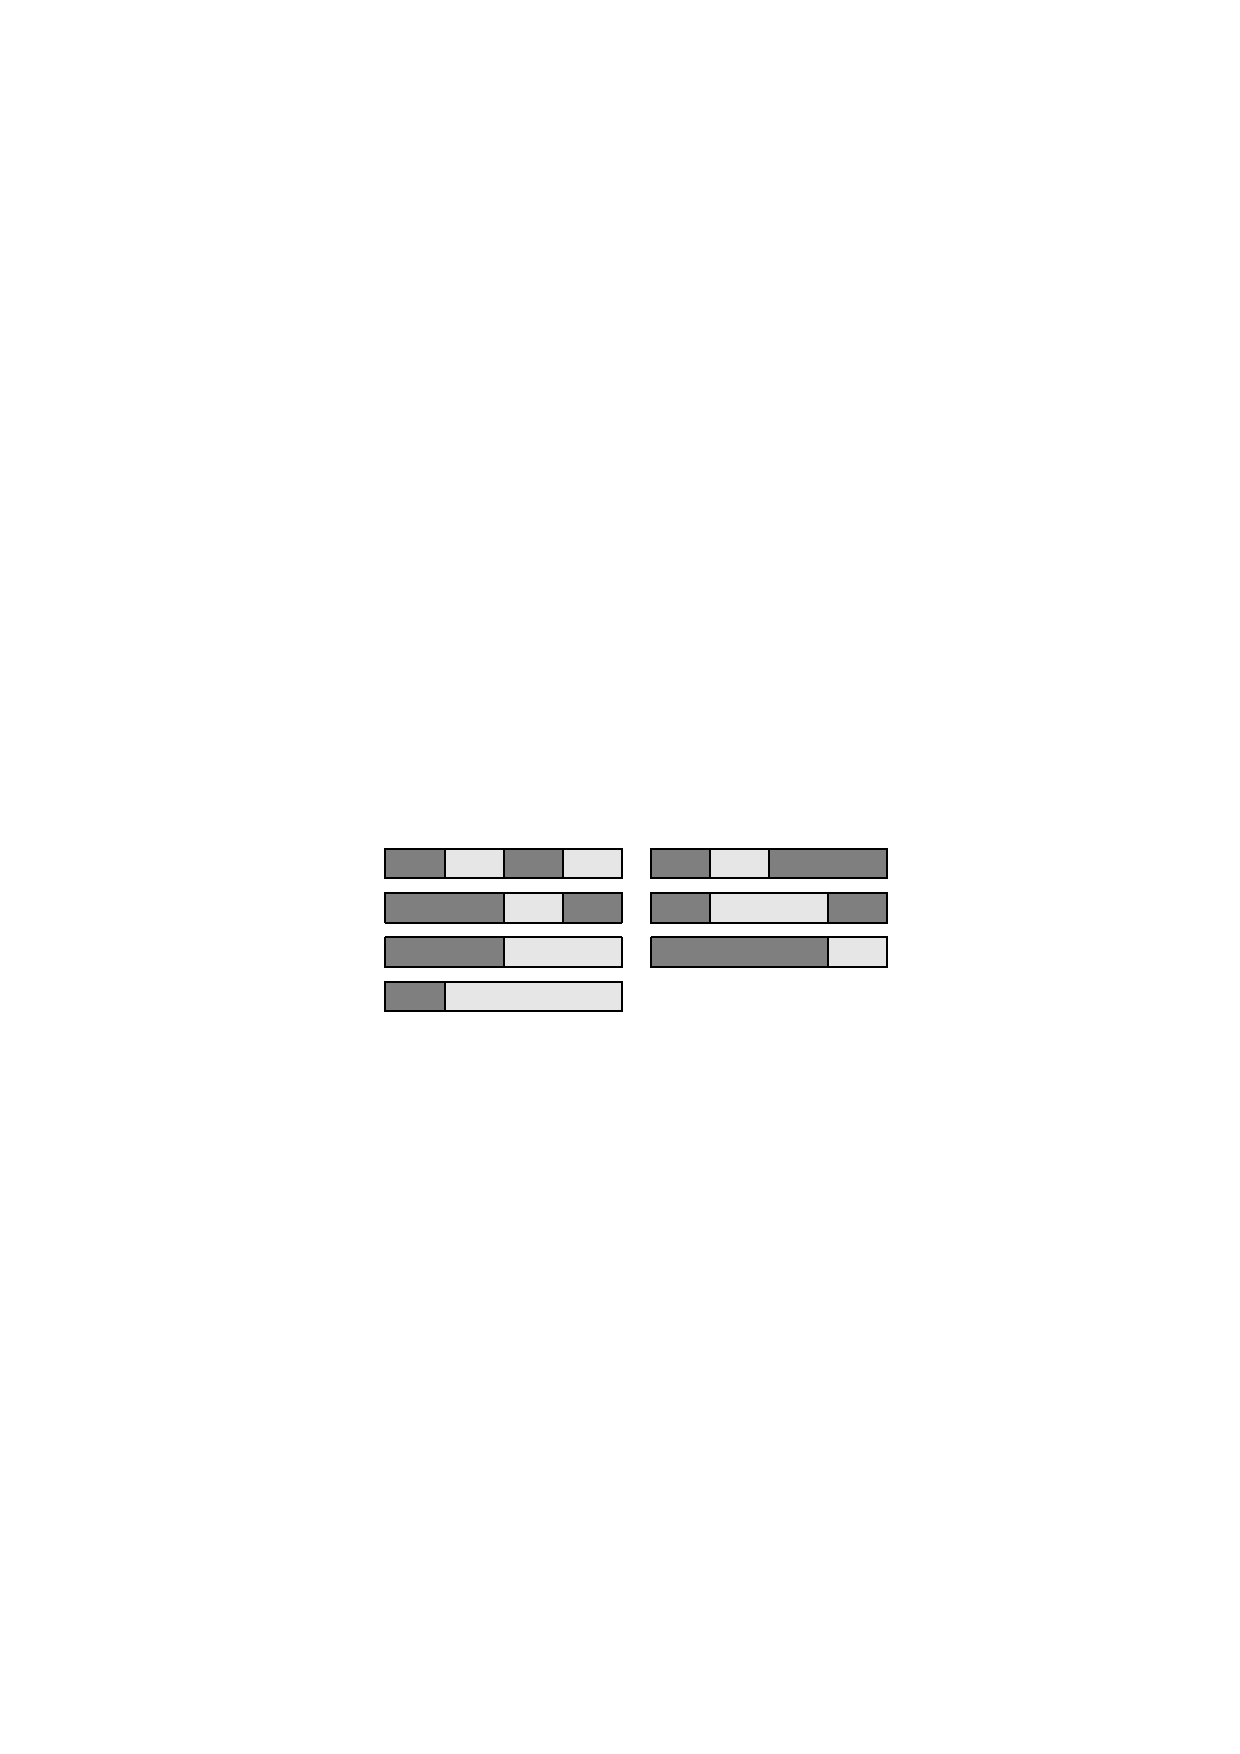
\includegraphics[width=0.9\textwidth]{plank.png}
    \caption{There are $7$ ways to glue together a $4$ meter plank.}
\end{figure}

If the plank should have length $n$ meters, in how many different ways can you glue pieces together to get a plank of the right length?

\section*{Input}
The first and only line of input contains an integer $n$ ($1 \le n \le 24$), the length of the new plank.

\section*{Output}
Output a single integer -- the number of ways you can glue together a plank of length $n$ meters.

\section*{Scoring}
Your solution will be tested on a set of test groups, each worth a number of points.
To get the points for a test group you need to solve all test cases in the test group. Your final score will be the maximum score of a single submission.

\noindent
\begin{tabular}{| l | l | l |}
  \hline
  Group & Points & Constraints \\ \hline
  $1$    & $33$        &  $n \le 10$ \\ \hline
  $2$    & $67$        &  No additional constraints \\ \hline
\end{tabular}
